% Provenance (never printed): see sources/outline_sources.md (Year 1: physical and chemical
% weathering; hydrolysis and its degrees; the ionic-potential diagram; clay minerals and
% climate; silicate weathering and carbon dioxide). Exercise and problem values in the Book 3
% scratch calculator calc/ch19.py; figure data from figdata/bachelor-1/ionic_potential.py and
% hydrolysis.py. Weathering is owned by Book 1 g5; chemical weathering, hydrolysis, clay mineral
% and laterite by Book 2 g10 (re-founded here). Silicate classes and the feldspars by ch. 7;
% Bowen's series by Book 2 g11; acid--base chemistry, solubility and oxidation by the chemistry
% books; soils and their horizons by the biology books. The silicate-weathering thermostat
% belongs to the Year 2 volume (told).
\chapter{Weathering and Clays}\label{ch:b1:weathering-clays}

The lettering of an old gravestone fades, the sharp edges of the letters
rounding off into shallow grooves, faster on a stone of marble than on one of
slate. A granite \omterm{def:b1:geological-maps:geological-map}{outcrop} that looks as hard as anything on Earth crumbles at
its surface into a gritty sand, which runs through the fingers as loose grains
of glassy quartz, chalky \omterm{def:b1:rock-forming-minerals:groups}{feldspar} and flakes of \omterm{def:b1:rock-forming-minerals:groups}{mica}. Under the forests of the
humid tropics, the solid rock may lie far down, below a red earth
that keeps the outlines of the rock's \omterm{def:b1:rock-forming-minerals:mineral}{minerals} but can be cut with a spade.
All three are the work of water at the Earth's surface. This chapter writes
that work as chemistry: which \omterm{def:b1:rock-forming-minerals:mineral}{minerals} give way first, what they become, why
some elements leave with the water and others stay, how the climate sets the
outcome, and how the slow decay of silicate rock draws carbon dioxide out of
the air.

\begin{recall}
Weathering breaks rocks down where they lie (Book~1, grade~5). \omterm{def:b1:weathering-clays:weathering}{Chemical
weathering} transforms the \omterm{def:b1:rock-forming-minerals:mineral}{minerals}; the \omterm{def:b1:weathering-clays:hydrolysis}{hydrolysis} of a \omterm{def:b1:rock-forming-minerals:groups}{feldspar} gives a \omterm{def:b1:weathering-clays:clay-mineral}{clay
mineral}, \omterm{def:b1:weathering-clays:clay-mineral}{kaolinite}, and sends potassium and silica to the rivers; a \omterm{def:b1:weathering-clays:laterite}{laterite} is
the red, iron- and aluminium-rich product of hot, wet climates (Book~2,
grade~10). Silicates are classified by how their \ce{SiO4} tetrahedra share
corners, a \omterm{def:b1:rock-forming-minerals:silicate-classes}{phyllosilicate} forming sheets; \omterm{def:b1:rock-forming-minerals:groups}{feldspars} are framework silicates of
sodium, potassium and calcium, \omterm{def:b1:rock-forming-minerals:groups}{micas} sheet silicates with potassium between the
sheets (\cref{def:b1:rock-forming-minerals:silicate-classes},
\cref{def:b1:rock-forming-minerals:groups}). The ionic radius of an ion depends on
its charge and on its coordination (\cref{ch:b1:rock-forming-minerals}). \omterm{def:b1:rock-forming-minerals:mineral}{Minerals}
crystallise from a cooling magma in the order of Bowen's reaction series,
\omterm{def:b1:rock-forming-minerals:groups}{olivine} first and quartz last (Book~2, grade~11). An acid releases hydrogen
ions; carbon dioxide dissolved in water forms carbonic acid; an oxidation is a
loss of electrons; a balanced equation conserves each element and the charge
(the chemistry books). A soil is a living layer organised into horizons (the
biology books).
\end{recall}

\section{Physical and chemical weathering}\label{sec:b1:weathering-clays:types}

A rock formed at depth, at high temperature and pressure and without free water
or oxygen, is out of equilibrium at the surface. It adjusts in two ways, which
work together.

\begin{definition}[Physical weathering, chemical weathering]\label{def:b1:weathering-clays:weathering}
\emph{Physical weathering}\index{physical weathering} is the breakdown of a
rock in place into smaller fragments without change of its \omterm{def:b1:rock-forming-minerals:mineral}{minerals}.
\emph{Chemical weathering}\index{chemical weathering} is the transformation of
the \omterm{def:b1:rock-forming-minerals:mineral}{minerals} of a rock in place by reaction with water and the substances it
carries, mainly hydrogen ions, dissolved carbon dioxide and oxygen: some
\omterm{def:b1:rock-forming-minerals:mineral}{minerals} dissolve, others are replaced by new \omterm{def:b1:rock-forming-minerals:mineral}{minerals} stable at the surface,
and part of the rock leaves in solution.
\end{definition}
% ledger: formoso:weathering

\emph{Frost.} Water at \qty{0}{\celsius} has the density
\qty{999.87}{kg.m^{-3}}, ice \qty{916.72}{kg.m^{-3}}: water expands by
\qty{9.1}{\percent} when it freezes. The old picture of frost weathering is
water freezing in a sealed crack and forcing it open, again at each thaw and
freeze. A model of cracks in granite and marble, built on fracture mechanics
and on what is known of freezing soils, puts the weight elsewhere: water is
drawn through the pores toward ice already in a crack, as it is toward the
ice lenses of a freezing soil, and the ice grows and wedges the crack as long
as the freezing lasts. Sustained freezing is most effective between about
\qty{-4}{\celsius} and \qty{-15}{\celsius}: closer to zero the ice cannot
build up enough pressure, and colder the water can no longer move to it.
% ledger: usgs:water-density, iapws:ice-density, wh85:frost

\emph{Heating, unloading and salt.} Repeated heating and cooling fatigue a
rock whose \omterm{def:b1:rock-forming-minerals:mineral}{minerals} expand by different amounts; a granite brought to the
surface by erosion, relieved of the weight above it, expands and splits into
sheets parallel to the surface; salts crystallising from evaporating water,
in deserts and on coasts, pry grains apart.

\omterm{def:b1:weathering-clays:weathering}{Physical weathering} does more than break rock: it opens it to water.

\begin{proposition}[The surface opened by fragmentation]\label{prop:b1:weathering-clays:surface}
A cube of side $L$ cut into cubes of side $L/n$ has $n$ times the surface
area. More generally, a mass $m$ of grains of density $\rho$, all cubes of side
$d$, has the surface area $S = 6m/(\rho d)$: the specific surface $S/m =
6/(\rho d)$ is inversely proportional to the grain size.
\end{proposition}

\begin{proof}
A cube of side $d$ has the area $6d^2$ and the mass $\rho d^3$, so the
specific surface of each grain, and of any number of them, is $6d^2/(\rho d^3)
= 6/(\rho d)$. Cutting a cube of side $L$ into $n^3$ cubes of side $L/n$ keeps
the mass and divides $d$ by $n$, which multiplies the area by $n$.
\end{proof}

A block of \omterm{def:b1:rock-forming-minerals:groups}{feldspar} of density about \qty{2600}{kg.m^{-3}} has a specific
surface of \qty{0.23}{m^2.kg^{-1}} as centimetre fragments, and
\qty{2.3}{m^2.g^{-1}} as micrometre grains, ten thousand times more. Chemical
reactions proceed at surfaces, so a rock shattered by frost or opened along
its joints weathers chemically much faster than the same rock intact.
% ledger: hom:albite, hom:orthoclase

\emph{The chemical reactions.} Calcite dissolves completely in water that
carries carbon dioxide, which is why marble gravestones lose their lettering
(Book~2, grade~10). Iron(II) of the dark silicates is oxidised to iron(III),
which stays as yellow-brown and red oxides. Most important by far, because
silicates make most of the \omterm{def:b1:layered-earth:layers}{crust}, is \omterm{def:b1:weathering-clays:hydrolysis}{hydrolysis}. The hydrogen ions come from
carbon dioxide, dissolved from the air and breathed out by roots and
decomposers into the soil, and from the organic acids of decaying plants:
unpolluted surface and soil waters have a pH between 5.5 and 7, and the water
of the organic layer of some forest soils as low as 3.5. Water, temperature,
surface area and acidity are thus the four controls of \omterm{def:b1:weathering-clays:weathering}{chemical weathering},
and a warm, wet climate with a thick soil provides all four.
% ledger: formoso:weathering

\section{The hydrolysis of silicates}\label{sec:b1:weathering-clays:hydrolysis}

\begin{definition}[Hydrolysis of a silicate]\label{def:b1:weathering-clays:hydrolysis}
The \emph{hydrolysis}\index{hydrolysis (of silicates)} of a silicate is its
reaction with water and hydrogen ions in which the hydrogen ions replace the
metal cations, which go into solution, part or all of the silicon leaves as
dissolved silicic acid \ce{H4SiO4}, and the rest of the \omterm{def:b1:rock-forming-minerals:mineral}{mineral} is rebuilt into
a new solid, a \omterm{def:b1:weathering-clays:clay-mineral}{clay mineral} or a hydroxide. The dissolution is incongruent:
the solid left does not have the composition of the \omterm{def:b1:rock-forming-minerals:mineral}{mineral} attacked.
\end{definition}
% ledger: formoso:weathering

Aluminium is the key to writing the reaction: at the pH of soils and rivers it
is almost insoluble, and the solid product keeps it all. Everything else
follows from that.

\begin{method}[Balancing a hydrolysis reaction]\label{met:b1:weathering-clays:balance}
Given the \omterm{def:b1:rock-forming-minerals:mineral}{mineral} attacked and the solid product:
\begin{enumerate}
  \item Take one formula unit of the product, and as much of the \omterm{def:b1:rock-forming-minerals:mineral}{mineral} as
        brings the same number of aluminium atoms.
  \item The silicon of the \omterm{def:b1:rock-forming-minerals:mineral}{mineral} not used by the product leaves as
        \ce{H4SiO4}; the metal cations not used by the product leave as ions.
  \item Balance the charge of these cations with hydrogen ions on the left.
  \item Balance the oxygen with water on the left.
  \item Check the hydrogen: it must balance by itself. If it does not, a
        formula is wrong.
  \item If a whole-number equation is wanted, multiply through.
\end{enumerate}
\end{method}

\begin{proposition}[Hydrolysis of the feldspars]\label{prop:b1:weathering-clays:feldspars}
With the \omterm{def:b1:weathering-clays:clay-mineral}{smectite} beidellite \ce{Na_{0.5}Al2(Si_{3.5}Al_{0.5})O10(OH)2}
(interlayer water left out), \omterm{def:b1:weathering-clays:clay-mineral}{kaolinite} \ce{Al2Si2O5(OH)4} and gibbsite
\ce{Al(OH)3} as products,
\begin{align*}
&\ce{5 NaAlSi3O8 + 4 H+ + 16 H2O -> 2 Na_{0.5}Al2(Si_{3.5}Al_{0.5})O10(OH)2 + 4 Na+ + 8 H4SiO4},\\ % ce-unbalanced-ok: decimal subscripts the checker cannot read; balance tested in tests/bachelor-1/test_weathering_clays.py
&\ce{2 NaAlSi3O8 + 2 H+ + 9 H2O -> Al2Si2O5(OH)4 + 2 Na+ + 4 H4SiO4},\\
&\ce{NaAlSi3O8 + H+ + 7 H2O -> Al(OH)3 + Na+ + 3 H4SiO4},\\
&\ce{CaAl2Si2O8 + 2 H+ + H2O -> Al2Si2O5(OH)4 + Ca^2+}.
\end{align*}
The albite loses \qty{80}{\percent} of its sodium and $8/15$ of its silicon to
the solution in the first reaction, all its sodium and $2/3$ of its silicon in
the second, all of both in the third. The anorthite loses all its calcium and
none of its silicon.
\end{proposition}
% ledger: webmineral:clays-b19, hom:albite, hom:anorthite

\begin{proof}
Apply the method. First reaction: two beidellite units hold $2\times2.5 = 5$
aluminium, the aluminium of 5 albite; the 15 silicon of the albite minus the
$2\times3.5 = 7$ of the product leave 8 \ce{H4SiO4}; the 5 sodium minus 1 leave
4 \ce{Na+}, balanced by 4 \ce{H+}; oxygen, $40 + w$ on the left and $24 + 32 =
56$ on the right, gives $w = 16$; hydrogen, $4 + 32 = 36$ and $4 + 32 = 36$,
checks. Second: 2 albite give the 2 aluminium of \omterm{def:b1:weathering-clays:clay-mineral}{kaolinite}, $6 - 2 = 4$
\ce{H4SiO4}, 2 \ce{Na+} and 2 \ce{H+}; oxygen $16 + w = 9 + 16$ gives $w = 9$;
hydrogen $2 + 18 = 20 = 4 + 16$. Third: one albite, three silicic acids, one
\ce{Na+} and one \ce{H+}; oxygen $8 + w = 3 + 12$ gives $w = 7$; hydrogen
$1 + 14 = 15 = 3 + 12$. Fourth: the 2 aluminium and 2 silicon of anorthite are
exactly those of \omterm{def:b1:weathering-clays:clay-mineral}{kaolinite}, no silicic acid leaves, \ce{Ca^2+} needs 2 \ce{H+};
oxygen $8 + w = 9$ gives $w = 1$; hydrogen $2 + 2 = 4$. The fractions exported
are the ions in solution over the atoms in the \omterm{def:b1:rock-forming-minerals:mineral}{mineral}: $4/5$ and $8/15$, then
$2/2$ and $4/6$, then $1/1$ and $3/3$.
\end{proof}

The same albite can thus give three different solids, and which one it gives
depends on how much water passes through the rock and carries the products
away: little water, and much of the silica and some of the cations stay to
build a \omterm{def:b1:weathering-clays:clay-mineral}{smectite}; more, and only enough silica for \omterm{def:b1:weathering-clays:clay-mineral}{kaolinite} stays; a great
deal, and the silica leaves entirely.

\begin{definition}[Bisiallitisation, monosiallitisation, allitisation]\label{def:b1:weathering-clays:hydrolysis-degree}
The degree of the \omterm{def:b1:weathering-clays:hydrolysis}{hydrolysis} of silicates is named after its product.
\emph{Bisiallitisation}\index{bisiallitisation} forms 2:1 \omterm{def:b1:weathering-clays:clay-mineral}{clay minerals}, such as
\omterm{def:b1:weathering-clays:clay-mineral}{smectites}, with about two silicon atoms per aluminium; part of the cations
stays in them. \emph{Monosiallitisation}\index{monosiallitisation} forms 1:1
\omterm{def:b1:weathering-clays:clay-mineral}{clay minerals}, \omterm{def:b1:weathering-clays:clay-mineral}{kaolinite}, with one silicon per aluminium; all the alkali and
alkaline-earth cations leave. \emph{Allitisation}\index{allitisation} removes
the silicon entirely and leaves aluminium hydroxide, gibbsite.
\end{definition}
% ledger: pedron:stages, formoso:weathering

The degree reached is a matter of climate first, through the rain and the
temperature, and then of the drainage of the profile. Where the water is
little renewed, a granite loses much of its sodium and calcium, potassium more
slowly, and only part of its silica: its \omterm{def:b1:rock-forming-minerals:groups}{feldspars} turn into 2:1 clays, and
much quartz is left; the rock falls apart into a sand of quartz, \omterm{def:b1:rock-forming-minerals:groups}{mica} and
half-weathered \omterm{def:b1:rock-forming-minerals:groups}{feldspar} mixed with clay. Under the heavy rains of the humid
tropics, more than \qty{2000}{mm} a year, the cations and the silica are
leached far more, and \omterm{def:b1:weathering-clays:clay-mineral}{kaolinite}, Si/Al = 1, forms. Where the leaching is most
intense, even the silica of \omterm{def:b1:weathering-clays:clay-mineral}{kaolinite} goes, and gibbsite remains.
% ledger: pedron:stages, goldich:1938, formoso:laterite

\begin{omfigure}
\begin{tikzpicture}[font=\small]
% fractions of albite's Na and Si exported by the three degrees (figdata/bachelor-1/hydrolysis.py)
\begin{axis}[width=10.5cm, height=6cm, ybar, bar width=0.5cm, ymin=0, ymax=112,
    xmin=0.45, xmax=3.55, xtick={1,2,3},
    xticklabels={{bisiallitisation\\ to beidellite\\ (Si/Al = 1.4)}, {monosiallitisation\\ to kaolinite\\ (Si/Al = 1)}, {allitisation\\ to gibbsite\\ (Si/Al = 0)}},
    xticklabel style={align=center, font=\footnotesize},
    ylabel={exported in solution (\si{\percent})}, ytick={0,20,...,100},
    legend style={at={(0.5,1.03)}, anchor=south, font=\footnotesize, legend columns=2, draw=none},
    nodes near coords={\pgfmathprintnumber[fixed,precision=0]{\pgfplotspointmeta}}, every node near coord/.append style={font=\scriptsize},
    enlarge x limits=false]
  \addplot[fill=omThm!60, draw=omThm!80!black] table[x=degree, y=Na] {figdata/out/bachelor-1-hydrolysis-degrees.dat};
  \addplot[fill=omDef!55, draw=omDef!80!black] table[x=degree, y=Si] {figdata/out/bachelor-1-hydrolysis-degrees.dat};
  \legend{sodium, silicon}
\end{axis}
\end{tikzpicture}

{\small The three degrees of \omterm{def:b1:weathering-clays:hydrolysis}{hydrolysis} of albite: the percentage of its sodium
and of its silicon carried away in solution, computed from the balanced
reactions, and the silicon to aluminium ratio of the solid left. The aluminium
stays entirely in the solid in all three.}
\label{fig:b1:weathering-clays:degrees}
\end{omfigure}


\begin{omfigure}
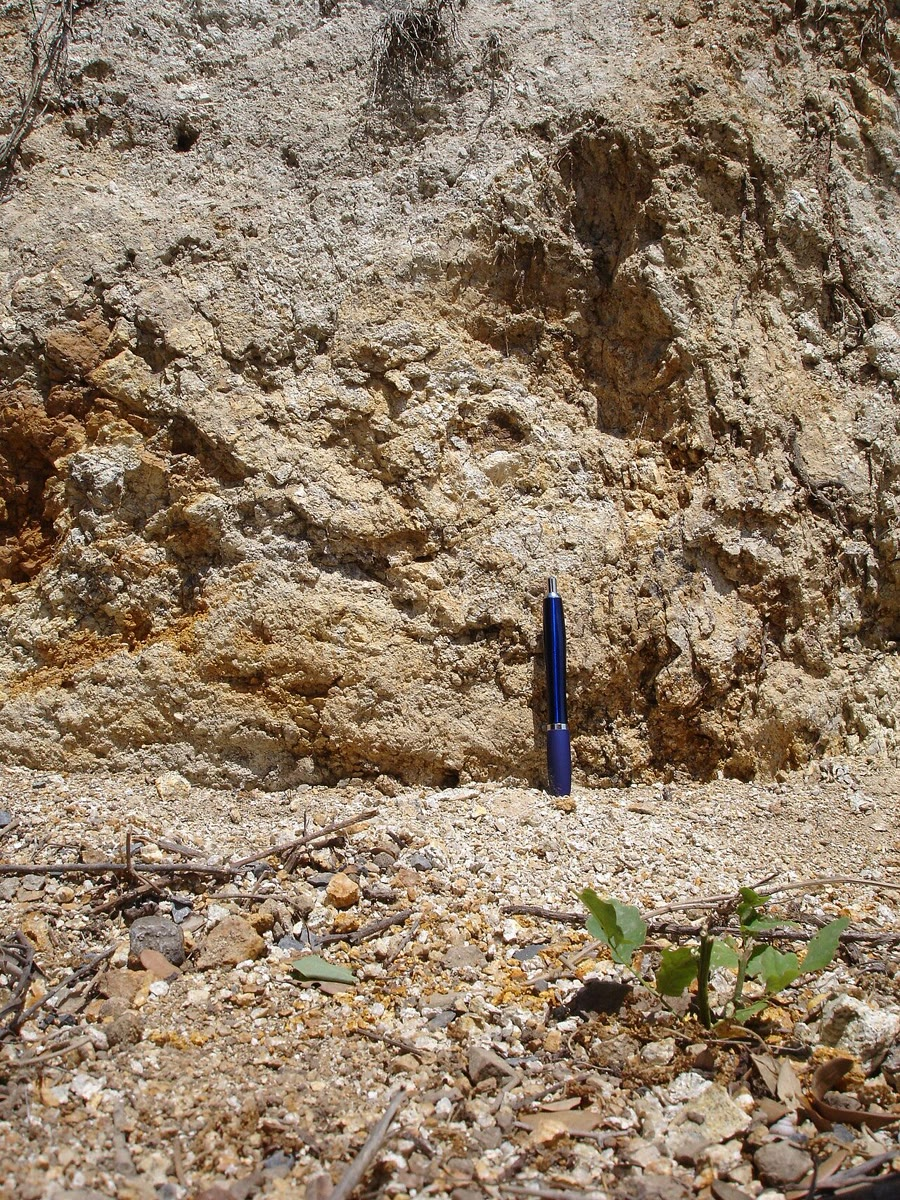
\includegraphics[height=6.3cm]{images/book3/b1-granite-grus.jpg}\hfill
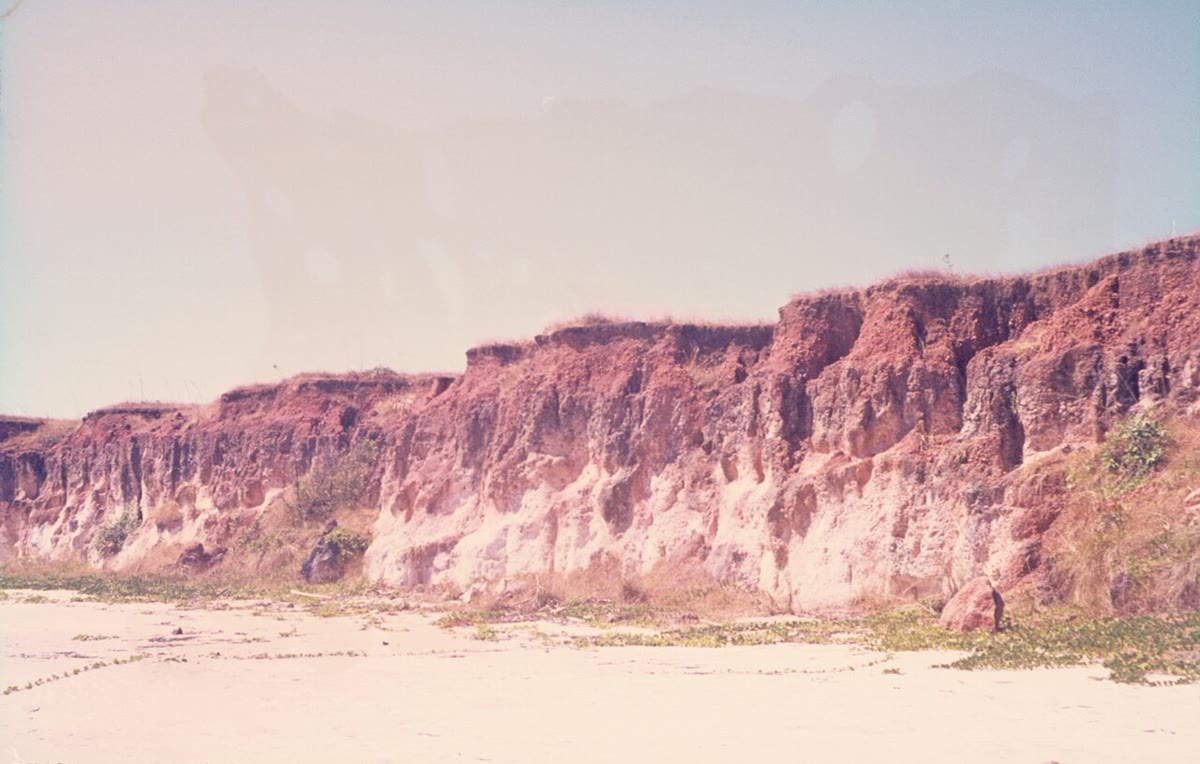
\includegraphics[height=6.3cm]{images/book3/b1-bauxite-weipa.jpg}
\par\smallskip{\small Left: rotten granite in the Pyrenees, still in place but
crumbling into a sand of quartz, \omterm{def:b1:rock-forming-minerals:groups}{feldspar} and \omterm{def:b1:rock-forming-minerals:groups}{mica}, with the loose sand at its
foot; the pen gives the scale. Photograph: Pinpin, CC~BY~2.5. Right: a
weathering profile on the coast at Weipa, northern Australia: red bauxite, the
product of \omterm{def:b1:weathering-clays:hydrolysis-degree}{allitisation}, over a white kaolinite-rich sandstone. Photograph:
Werner Schellmann, 1969, CC~BY-SA~2.5. Both from Wikimedia Commons.}
\label{fig:b1:weathering-clays:photos}
\end{omfigure}
% ledger: commons:grus, commons:weipa

\emph{Which \omterm{def:b1:rock-forming-minerals:mineral}{minerals} go first.} In 1938 Samuel Goldich, comparing weathered
profiles with their parent rocks, proposed a series of the \omterm{def:b1:rock-forming-minerals:mineral}{minerals} from the
least to the most stable in weathering, and found that it follows the order
in which they crystallise from a magma: \omterm{def:b1:rock-forming-minerals:groups}{olivine} and calcium-rich \omterm{def:b1:rock-forming-minerals:groups}{plagioclase}
first, quartz last. The \omterm{def:b1:rock-forming-minerals:mineral}{minerals} formed at the highest temperatures are the
furthest from equilibrium at the surface. A modern list, from the least to the
most resistant, reads: pyrite, calcite, dolomite, \omterm{def:b1:rock-forming-minerals:groups}{olivine}, calcium
\omterm{def:b1:rock-forming-minerals:groups}{plagioclase}, \omterm{def:b1:rock-forming-minerals:groups}{pyroxenes}, intermediate \omterm{def:b1:rock-forming-minerals:groups}{plagioclase}, \omterm{def:b1:rock-forming-minerals:groups}{amphiboles}, biotite,
potassium \omterm{def:b1:rock-forming-minerals:groups}{feldspar}, muscovite, \omterm{def:b1:weathering-clays:clay-mineral}{smectite}, quartz, \omterm{def:b1:weathering-clays:clay-mineral}{kaolinite}, and the oxides
gibbsite and hematite. Laboratory measurements of dissolution rates confirm
the ranking; it remains a ranking, not a law, since the rate of each \omterm{def:b1:rock-forming-minerals:mineral}{mineral}
also depends on the water around it. The end products of weathering,
\omterm{def:b1:weathering-clays:clay-mineral}{kaolinite}, gibbsite and hematite, are the most resistant of all: they are
already stable at the surface.
% ledger: goldich:1938, formoso:weatherability, lasaga:1984

\emph{The balance of a weathering profile.} Weathering removes matter, so a
concentration measured in a weathered rock does not tell how much was lost:
the loss of other elements concentrates those that stay. An element that does
not move gives the reference.

\begin{proposition}[Mass balance with an immobile element]\label{prop:b1:weathering-clays:immobile}
Let $i$ be an element that weathering does not move, with mass fractions
$C_{i,p}$ in the parent rock and $C_{i,w}$ in the weathered rock. Then a mass
$m_p$ of parent rock becomes the mass $m_w = m_p C_{i,p}/C_{i,w}$ of weathered
rock, and the fraction of any other element $j$ lost is
\[
  f_j = 1 - \frac{C_{j,w}}{C_{j,p}}\,\frac{C_{i,p}}{C_{i,w}} .
\]
\end{proposition}

\begin{proof}
The mass of $i$ is conserved: $m_p C_{i,p} = m_w C_{i,w}$, which gives $m_w$.
The mass of $j$ goes from $m_p C_{j,p}$ to $m_w C_{j,w}$, a fraction
$m_w C_{j,w}/(m_p C_{j,p}) = (C_{j,w}/C_{j,p})(C_{i,p}/C_{i,w})$ of it
remaining; $f_j$ is one minus this fraction.
\end{proof}

Titanium and zirconium are the usual choices, for a reason the next section
gives.

\section{Which elements leave: the ionic potential}\label{sec:b1:weathering-clays:ionic}

Sodium, potassium and calcium leave with the water; aluminium, iron(III) and
titanium stay; silicon is in between. The difference lies in how each ion
behaves in water.

\begin{definition}[Ionic potential]\label{def:b1:weathering-clays:ionic-potential}
The \emph{ionic potential}\index{ionic potential} of an ion is the ratio $z/r$
of its charge number $z$ to its ionic radius $r$, here in ångströms (for the
same coordination for all ions, sixfold in what follows).
\end{definition}
% ledger: nomad:goldschmidt, dangic:goldschmidt, shannon:radii-b19

\begin{proposition}[The three fields of the ionic potential]\label{prop:b1:weathering-clays:fields}
In the water of weathering, ions with $z/r < 3$ stay in solution as hydrated
cations and are carried away (soluble cations); ions with $3 < z/r < 10$ bind
the hydroxide ions of water and precipitate as hydroxides or oxides where they
are released (hydrolysates); ions with $z/r > 10$ bind oxygen so strongly that
they repel the hydrogen ions and travel as soluble oxyanions, such as
carbonate, sulfate, phosphate and nitrate. Silicon, at $z/r = 10$, lies on the
boundary, and is leached in part, more the more intense the weathering.
\end{proposition}
\admitted
% ledger: nomad:goldschmidt, dangic:goldschmidt

The rule is empirical, due to Victor Moritz Goldschmidt in the 1930s, and its
boundaries are approximate; the chemistry behind it, the attraction between a
cation and the oxygen of the water molecules around it, belongs to the
chemistry books. A small, highly charged cation pulls the electrons of its
water molecules so hard that they lose a hydrogen ion and become hydroxide:
moderately, and the hydroxide precipitates; extremely, and even the hydroxide
loses its hydrogen, leaving an oxyanion.

The diagram below reads the weathering of a rock at a glance. Sodium ($z/r = 0.98$),
potassium (0.72), calcium (2.0) and magnesium (2.8) leave: they are the
cations of river and sea water. Aluminium (5.6), iron(III) (4.7), titanium
(6.6) and zirconium (5.6) stay, and accumulate in the most weathered profiles;
titanium and zirconium, which in addition sit in \omterm{def:b1:rock-forming-minerals:mineral}{minerals} that hardly weather,
are the immobile references of \cref{prop:b1:weathering-clays:immobile}. Silicon
(10.0) is the element whose partial loss defines the degrees of \omterm{def:b1:weathering-clays:hydrolysis}{hydrolysis}.
% ledger: shannon:radii-b19

Oxidation moves an ion across the boundary. Iron(II), with $z/r = 2.6$, is a
soluble cation; iron(III), at 4.7, a hydrolysate. In a waterlogged soil
without oxygen, iron dissolves as \ce{Fe^2+} and is carried away, leaving grey
soil; where the water meets air, at a spring or in a well-drained soil, the
iron is oxidised and precipitates at once as red and brown oxides. Manganese
behaves the same way, \ce{Mn^2+} (2.4) against \ce{Mn^4+} (7.5).
% ledger: nomad:goldschmidt, shannon:radii-b19

\begin{omfigure}
\begin{tikzpicture}[font=\small]
% ionic-potential diagram (figdata/bachelor-1/ionic_potential.py): charge against Shannon radius
\begin{axis}[width=12.5cm, height=8.4cm, xmin=0, xmax=1.8, ymin=0, ymax=7,
    xlabel={ionic radius $r$ (\si{\angstrom}, sixfold coordination)}, ylabel={charge $z$},
    ytick={1,...,6}, xtick={0,0.2,...,1.8}, xticklabel style={/pgf/number format/fixed},
    axis on top, clip=true]
  \fill[omThm!14] (axis cs:0,0) -- (axis cs:1.8,0) -- (axis cs:1.8,5.4) -- cycle;
  \fill[omDef!16] (axis cs:0,0) -- (axis cs:1.8,5.4) -- (axis cs:1.8,7) -- (axis cs:0.7,7) -- cycle;
  \fill[omExo!18] (axis cs:0,0) -- (axis cs:0.7,7) -- (axis cs:0,7) -- cycle;
  \addplot[black, thick] table[x=r, y=z3] {figdata/out/bachelor-1-ionic_potential-lines.dat};
  \addplot[black, thick] table[x=r, y=z10] {figdata/out/bachelor-1-ionic_potential-lines.dat};
  \addplot[only marks, mark=*, mark size=1.6pt, black,
      point meta=explicit symbolic, nodes near coords,
      visualization depends on={value \thisrow{anc} \as \anc},
      every node near coord/.append style={font=\scriptsize, inner sep=2.6pt, anchor=\anc}]
    table[x=r, y=z, meta=tex] {figdata/out/bachelor-1-ionic_potential-ions.dat};
  \node[font=\footnotesize, align=center, fill=white, fill opacity=0.8, text opacity=1, rounded corners=1pt] at (axis cs:1.45,2.75) {soluble cations\\ $z/r < 3$};
  \node[font=\footnotesize, align=center, fill=white, fill opacity=0.8, text opacity=1, rounded corners=1pt] at (axis cs:1.15,6.3) {hydrolysates\\ $3 < z/r < 10$};
  \node[font=\footnotesize, align=left, fill=white, fill opacity=0.8, text opacity=1, rounded corners=1pt, anchor=north west] at (axis cs:0.015,6.95) {soluble oxyanions, $z/r > 10$};
  \node[font=\scriptsize, rotate=28, anchor=south] at (axis cs:1.62,4.86) {$z/r = 3$};
  \node[font=\scriptsize, rotate=61, anchor=south] at (axis cs:0.2,2.0) {$z/r = 10$};
\end{axis}
\end{tikzpicture}

{\small The ionic-potential diagram: each ion placed by its effective ionic
radius in sixfold coordination (Shannon, 1976) and its charge. The lines
$z/r = 3$ and $z/r = 10$ separate the ions that leave in solution as cations,
those that stay as hydroxides or oxides, and those that leave as oxyanions.
Silicon lies on the upper boundary.}
\label{fig:b1:weathering-clays:ionic-potential}
\end{omfigure}
% ledger: shannon:radii-b19, nomad:goldschmidt

\section{Clay minerals}\label{sec:b1:weathering-clays:clays}

\begin{definition}[Clay mineral, kaolinite, illite, smectite, chlorite]\label{def:b1:weathering-clays:clay-mineral}
A \emph{clay mineral}\index{clay mineral} is a hydrous aluminium
\omterm{def:b1:rock-forming-minerals:silicate-classes}{phyllosilicate}, usually in grains a few micrometres across or less, built of
layers that combine a tetrahedral sheet (T) of \ce{SiO4} tetrahedra sharing
three corners and an octahedral sheet (O) of aluminium or magnesium surrounded
by oxygen and hydroxyl. In \emph{kaolinite}\index{kaolinite},
\ce{Al2Si2O5(OH)4}, each layer is one T and one O sheet (a 1:1 or T--O layer),
uncharged, and the layers are held by hydrogen bonds. In the 2:1 or T--O--T
clay \omterm{def:b1:rock-forming-minerals:mineral}{minerals} an O sheet lies between two T sheets pointing toward it:
\emph{illite}\index{illite} is a non-expanding 2:1 clay \omterm{def:b1:rock-forming-minerals:mineral}{mineral} with potassium
ions between the layers, like a \omterm{def:b1:rock-forming-minerals:groups}{mica} with less potassium;
a \emph{smectite}\index{smectite} is a 2:1 clay \omterm{def:b1:rock-forming-minerals:mineral}{mineral} with hydrated,
exchangeable cations and water between its layers, which can take up more
water and swell; a \emph{chlorite}\index{chlorite} is a 2:1 \omterm{def:b1:rock-forming-minerals:mineral}{mineral} whose
negatively charged layers alternate with positively charged octahedral sheets
of brucite type, \ce{(Mg,Fe)(OH)2} with some aluminium.
\end{definition}
% ledger: usgs:clay-groups, usgs:clay-settings, webmineral:clays-b19, biscaye:1965

The charge of a layer decides how the layers stack, and the charge comes from
substitutions in the sheets (\cref{def:b1:rock-forming-minerals:substitution}).

\begin{proposition}[Charge of a 2:1 layer]\label{prop:b1:weathering-clays:layer-charge}
A 2:1 layer of formula $\mathrm{(Si_{4-x}Al_x)(Al_{2-y}Mg_y)O_{10}(OH)_2}$, with
$x$ aluminium for silicon in its tetrahedral sheets and $y$ magnesium for
aluminium in its octahedral sheet, carries the charge $-(x + y)$ per formula
unit.
\end{proposition}

\begin{proof}
Add the charges: $4(4 - x) + 3x$ from the tetrahedral cations, $3(2 - y) + 2y$
from the octahedral ones, $-2\times10$ from the oxygens and $-1\times2$ from the
hydroxyls: $16 - x + 6 - y - 20 - 2 = -(x + y)$.
\end{proof}

Without substitution ($x = y = 0$) the layer is neutral, as in
\ce{Al2Si4O10(OH)2}, the \omterm{def:b1:rock-forming-minerals:mineral}{mineral} pyrophyllite, and the layers are held only by
weak forces.
In muscovite, $x = 1$, a charge of $-1$ is balanced by one potassium ion that
locks the layers together; \omterm{def:b1:weathering-clays:clay-mineral}{illite} is close to it, with a little less. In the
beidellite of \cref{prop:b1:weathering-clays:feldspars}, $x = 0.5$: the charge
$-0.5$ is balanced by $0.5$ sodium. A smaller charge holds the layers less
tightly, and between them water and hydrated cations can enter: this is why
\omterm{def:b1:weathering-clays:clay-mineral}{smectites}, with charges of about 0.3 to 0.5 per formula unit, as in the
montmorillonite and beidellite formulas, swell, while \omterm{def:b1:weathering-clays:clay-mineral}{illite} does not. The
interlayer cations of a \omterm{def:b1:weathering-clays:clay-mineral}{smectite} are exchangeable, and the exchange capacity of
the common \omterm{def:b1:weathering-clays:clay-mineral}{clay minerals} follows their structure: 3 to 15 milliequivalents per
\qty{100}{g} for \omterm{def:b1:weathering-clays:clay-mineral}{kaolinite}, whose layers carry no charge, 10 to 40 for \omterm{def:b1:weathering-clays:clay-mineral}{illite},
70 to 100 for montmorillonite, a \omterm{def:b1:weathering-clays:clay-mineral}{smectite}. Potassium, which locks the layers
of a \omterm{def:b1:rock-forming-minerals:groups}{mica}, favours \omterm{def:b1:weathering-clays:clay-mineral}{illite}; \omterm{def:b1:weathering-clays:clay-mineral}{smectites} form where potassium is scarce and
calcium and magnesium are available.
% ledger: webmineral:clays-b19, carroll:cec, usgs:clay-settings

\begin{omfigure}
\begin{tikzpicture}[font=\footnotesize, >={Stealth[length=4pt]}, y=0.2cm, x=1cm]
% schematic clay-mineral structures, vertical scale proportional to the basal spacings
% (USGS OFR 01-041, ledger usgs:clay-xrd): kaolinite 7, illite 10, smectite 14 (air-dried), chlorite 14 angstrom.
% T sheet 2 A thick, O sheet 2.4 A thick (schematic); the column width is 2.2 cm.
\def\W{2.2}
\newcommand{\Tsheet}[1]{% tetrahedral sheet whose base is at y=#1
  \fill[omDef!35] (0,#1) rectangle (\W,#1+2);
  \foreach \i in {0,...,6} {\draw[omDef!80!black, line width=0.4pt] (0.04+\i*0.31,#1) -- (0.195+\i*0.31,#1+2) -- (0.35+\i*0.31,#1) -- cycle;}
}
\newcommand{\TsheetDown}[1]{% inverted tetrahedral sheet, base at the top (y=#1+2)
  \fill[omDef!35] (0,#1) rectangle (\W,#1+2);
  \foreach \i in {0,...,6} {\draw[omDef!80!black, line width=0.4pt] (0.04+\i*0.31,#1+2) -- (0.195+\i*0.31,#1) -- (0.35+\i*0.31,#1+2) -- cycle;}
}
\newcommand{\Osheet}[2]{% octahedral sheet, base at y=#1, fill colour #2
  \fill[#2] (0,#1) rectangle (\W,#1+2.4);
  \foreach \i in {0,...,4} {\draw[black!55, line width=0.4pt] (0.17+\i*0.42,#1+1.2) -- ++(0.17,1.0) -- ++(0.17,-1.0) -- ++(-0.17,-1.0) -- cycle;}
}
\newcommand{\spacing}[3]{% arrow for d001 from y=#1 to y=#2 with label #3
  \draw[<->, line width=0.5pt] (\W+0.18,#1) -- (\W+0.18,#2) node[midway, right, inner sep=2pt] {#3};
  \draw[black!40, densely dotted] (\W,#1) -- (\W+0.28,#1); \draw[black!40, densely dotted] (\W,#2) -- (\W+0.28,#2);
}
% ---------- kaolinite: T-O, d = 7.2
\begin{scope}[xshift=0cm]
  \foreach \b in {0, 7.2} {\Tsheet{\b} \Osheet{\b+2}{omThm!25}}
  \spacing{0}{7.2}{\SI{7}{\angstrom}}
  \node[anchor=north, align=center] at (\W/2,-0.8) {\textbf{kaolinite}\\ T--O (1:1) layers\\ held by hydrogen bonds};
\end{scope}
% ---------- illite: T-O-T + K, d = 10
\begin{scope}[xshift=3.6cm]
  \foreach \b in {0, 10} {\Tsheet{\b} \Osheet{\b+2}{omThm!25} \TsheetDown{\b+4.4}}
  \foreach \b in {6.4} {\foreach \i in {0,...,4} \fill[omExo!70!black] (0.25+\i*0.42,\b+1.8) circle[radius=1.5pt];}
  \spacing{0}{10}{\SI{10}{\angstrom}}
  \node[anchor=north, align=center] at (\W/2,-0.8) {\textbf{illite}\\ T--O--T (2:1) layers\\ held by \ce{K+} ions};
\end{scope}
% ---------- smectite: T-O-T + hydrated cations, d = 14
\begin{scope}[xshift=7.2cm]
  \foreach \b in {0, 14} {\Tsheet{\b} \Osheet{\b+2}{omThm!25} \TsheetDown{\b+4.4}}
  \foreach \i in {0,...,9} {\draw[omDef!60, line width=0.3pt] (0.13+\i*0.215,8.6) circle[radius=1.3pt]; \draw[omDef!60, line width=0.3pt] (0.2+\i*0.215,11.8) circle[radius=1.3pt];}
  \foreach \i in {0,...,3} {\fill[omExo!70!black] (0.35+\i*0.5,10.2) circle[radius=1.5pt];}
  \spacing{0}{14}{\SI{14}{\angstrom}}
  \node[anchor=north, align=center] at (\W/2,-0.8) {\textbf{smectite}\\ T--O--T layers, hydrated\\ \ce{Na+}, \ce{Ca^2+} and water};
\end{scope}
% ---------- chlorite: T-O-T + brucite-like O sheet, d = 14
\begin{scope}[xshift=10.8cm]
  \foreach \b in {0, 14} {\Tsheet{\b} \Osheet{\b+2}{omThm!25} \TsheetDown{\b+4.4}}
  \Osheet{9}{omExo!25}
  \spacing{0}{14}{\SI{14}{\angstrom}}
  \node[anchor=north, align=center] at (\W/2,-0.8) {\textbf{chlorite}\\ T--O--T layers and a\\ brucite-like O sheet};
\end{scope}
% key
\begin{scope}[xshift=0cm, yshift=-2.75cm]
  \fill[omDef!35] (0,0) rectangle (0.4,1.6); \draw[omDef!80!black] (0.05,0) -- (0.2,1.6) -- (0.35,0) -- cycle;
  \node[anchor=west] at (0.5,0.8) {T: tetrahedral sheet, \ce{SiO4} (some \ce{AlO4})};
  \fill[omExo!70!black] (8.1,0.8) circle[radius=1.5pt]; \node[anchor=west] at (8.3,0.8) {interlayer cation};
  \fill[omThm!25] (0,-2.6) rectangle (0.4,-1.0);
  \node[anchor=west] at (0.5,-1.8) {O: octahedral sheet, \ce{Al} or \ce{Mg} with \ce{O} and \ce{OH}};
  \draw[omDef!60] (8.1,-1.8) circle[radius=1.3pt]; \node[anchor=west] at (8.3,-1.8) {water molecule};
\end{scope}
\end{tikzpicture}

{\small The four families of \omterm{def:b1:weathering-clays:clay-mineral}{clay minerals} (schematic, two layers of each). The
vertical scale is proportional to the basal spacing, the repeat distance from
one layer to the next measured by X-ray diffraction: \SI{7}{\angstrom} for
\omterm{def:b1:weathering-clays:clay-mineral}{kaolinite}, \SI{10}{\angstrom} for \omterm{def:b1:weathering-clays:clay-mineral}{illite}, about \SI{14}{\angstrom} for an
air-dried \omterm{def:b1:weathering-clays:clay-mineral}{smectite} and for \omterm{def:b1:weathering-clays:clay-mineral}{chlorite}.}
\label{fig:b1:weathering-clays:structures}
\end{omfigure}
% ledger: usgs:clay-xrd, usgs:clay-groups



\begin{table}[htbp]
\centering\footnotesize
\setlength{\tabcolsep}{4pt}
% ledger: usgs:clay-xrd, usgs:clay-groups, usgs:clay-settings, carroll:cec, biscaye:1965
\begin{tabular}{@{}>{\raggedright\arraybackslash}p{1.6cm}>{\raggedright\arraybackslash}p{1.5cm}>{\raggedright\arraybackslash}p{1.6cm}>{\raggedright\arraybackslash}p{1.5cm}>{\raggedright\arraybackslash}p{1.4cm}>{\raggedright\arraybackslash}p{1.4cm}>{\raggedright\arraybackslash}p{1.2cm}>{\raggedright\arraybackslash}p{3.2cm}@{}}
\hline
\omterm{def:b1:rock-forming-minerals:mineral}{mineral} & layer & interlayer & air-dried & glycol & heated & CEC & typical setting \\
\hline
\omterm{def:b1:weathering-clays:clay-mineral}{kaolinite} & T--O & none & \SI{7}{\angstrom} & \SI{7}{\angstrom} & destroyed at \SI{550}{\celsius} & 3--15 & \omterm{def:b1:rock-forming-minerals:groups}{feldspars} leached by acid water; intense tropical weathering \\
\omterm{def:b1:weathering-clays:clay-mineral}{illite} & T--O--T & \ce{K+} & \SI{10}{\angstrom} & \SI{10}{\angstrom} & \SI{10}{\angstrom} & 10--40 & alkaline water rich in K; from \omterm{def:b1:rock-forming-minerals:groups}{feldspars} and \omterm{def:b1:rock-forming-minerals:groups}{micas}; the main clay of mudstones \\
\omterm{def:b1:weathering-clays:clay-mineral}{smectite} & T--O--T & hydrated \ce{Na+}, \ce{Ca^2+} & about \SI{14}{\angstrom} & \SI{17}{\angstrom} & \SI{10}{\angstrom} at \SI{400}{\celsius} & 70--100 & weathered basic rocks; poorly drained ground, K scarce \\
\omterm{def:b1:weathering-clays:clay-mineral}{chlorite} & T--O--T & brucite-like sheet & \SI{14}{\angstrom} & \SI{14}{\angstrom} & \SI{14}{\angstrom} & -- & low-grade metamorphic and altered igneous rocks; mudstones \\
\hline
\end{tabular}
\caption{The four \omterm{def:b1:rock-forming-minerals:mineral}{clay-mineral} families: structure, basal spacing measured on
oriented mounts air-dried, after solvation with ethylene glycol and after
heating, cation-exchange capacity (CEC, milliequivalents per \qty{100}{g}; the
value for \omterm{def:b1:weathering-clays:clay-mineral}{smectite} is that of montmorillonite) and
where they typically form.}
\label{tab:b1:weathering-clays:clays}
\end{table}

\begin{inthelab}[Identifying clay minerals by X-ray diffraction]
\omterm{def:b1:weathering-clays:clay-mineral}{Clay minerals} are too fine to be told apart under the optical microscope. In
the laboratory, the finest fraction of a soil or a mudstone is separated by
letting the coarser grains settle out of water, and a drop of the suspension is
dried on a glass slide, where the flakes lie flat: an oriented mount. X-rays
reflected by the stacked layers give strong peaks at the angles set by the
basal spacing, by Bragg's law of diffraction (physics). The slide is run three
or four times: air-dried; after a night in ethylene-glycol vapour, which enters
the interlayers of \omterm{def:b1:weathering-clays:clay-mineral}{smectites} and swells them to \SI{17}{\angstrom} while leaving
the other \omterm{def:b1:rock-forming-minerals:mineral}{minerals} unchanged; after heating to \SI{400}{\celsius}, which drives
the water out of \omterm{def:b1:weathering-clays:clay-mineral}{smectites} and collapses them to \SI{10}{\angstrom}; and after
heating to \SI{550}{\celsius}, which destroys \omterm{def:b1:weathering-clays:clay-mineral}{kaolinite} but leaves \omterm{def:b1:weathering-clays:clay-mineral}{illite} and
\omterm{def:b1:weathering-clays:clay-mineral}{chlorite}. \Cref{tab:b1:weathering-clays:clays} is the key to reading the four
runs; mixtures and interlayered \omterm{def:b1:rock-forming-minerals:mineral}{minerals}, very common in soils, need more.
\end{inthelab}
% ledger: usgs:clay-xrd

\begin{omfigure}
\begin{minipage}[t]{0.66\linewidth}\vspace{0pt}
\emph{Clays as climate indicators.} Because the degree of \omterm{def:b1:weathering-clays:hydrolysis}{hydrolysis} follows
the climate, the \omterm{def:b1:weathering-clays:clay-mineral}{clay minerals} of a soil record it: \omterm{def:b1:weathering-clays:clay-mineral}{kaolinite} and gibbsite
where weathering is intense, under hot, wet climates; \omterm{def:b1:weathering-clays:clay-mineral}{smectites} where the
water is little renewed; where weathering is weak, the clays are mostly
inherited from the rock, \omterm{def:b1:weathering-clays:clay-mineral}{illite} and \omterm{def:b1:weathering-clays:clay-mineral}{chlorite} from \omterm{def:b1:rock-forming-minerals:groups}{micas} and schists. Rivers
carry these clays to the sea, and the deep-sea muds keep the record: off the
small rivers of tropical South America, rich in \omterm{def:b1:weathering-clays:clay-mineral}{kaolinite} and gibbsite, they
show the intense weathering of the land they drain. When soils are buried and
preserved, their \omterm{def:b1:weathering-clays:clay-mineral}{clay minerals} are used to infer the climates of the
geological past: a bed rich in \omterm{def:b1:weathering-clays:clay-mineral}{kaolinite} in a sequence of illite-rich
mudstones points to a warm, wet episode. Such inference needs care, because
\omterm{def:b1:weathering-clays:clay-mineral}{clay minerals} are also transported far from where they formed, and are
transformed by burial, the \omterm{def:b1:weathering-clays:clay-mineral}{smectites} turning into \omterm{def:b1:weathering-clays:clay-mineral}{illite} as they are heated
(\cref{ch:b1:diagenesis-basins}).
\end{minipage}\hfill
\begin{minipage}[t]{0.30\linewidth}\vspace{0pt}
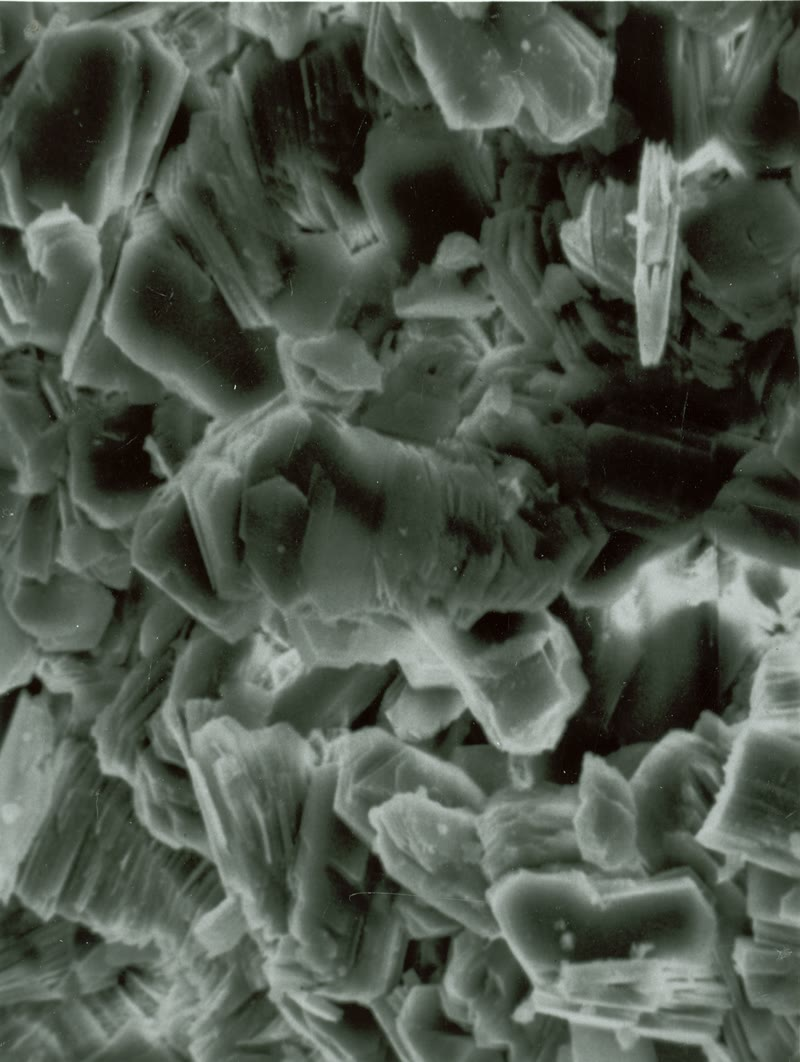
\includegraphics[width=\linewidth]{images/book3/b1-kaolinite-sem.jpg}

{\scriptsize \omterm{def:b1:weathering-clays:clay-mineral}{Kaolinite} seen with a scanning electron microscope: books of
stacked hexagonal plates grown in the pores of a sandstone of northern Alaska
(magnification about 1340). U.S. Geological Survey, public domain, via
Wikimedia Commons.\par}
\end{minipage}
\end{omfigure}
% ledger: biscaye:1965, usgs:clay-settings, pedron:stages, commons:kaolinite-sem

\emph{\omterm{def:b1:weathering-clays:laterite}{Laterites}.} Where \omterm{def:b1:weathering-clays:hydrolysis}{hydrolysis} reaches its last degrees for a long time,
the profile thickens and its top concentrates everything that does not leave.

\begin{definition}[Laterite]\label{def:b1:weathering-clays:laterite}
A \emph{laterite}\index{laterite} is the iron- and aluminium-rich product of
intense and prolonged \omterm{def:b1:weathering-clays:hydrolysis}{hydrolysis} under hot, wet climates: a red to brown
material, soft or hardened, made of \omterm{def:b1:weathering-clays:clay-mineral}{kaolinite} and iron oxides and hydroxides,
with gibbsite where \omterm{def:b1:weathering-clays:hydrolysis-degree}{allitisation} is reached, from which nearly all the alkali
and alkaline-earth cations and much of the silica have been removed.
\end{definition}
% ledger: formoso:laterite, buchanan:laterite

A \omterm{def:b1:weathering-clays:laterite}{laterite} rich enough in gibbsite or boehmite, the aluminium hydroxides, is a
bauxite, the ore of nine-tenths of the aluminium: \omterm{def:b1:weathering-clays:hydrolysis-degree}{allitisation} is the step that
makes the ore. Most bauxites are residual, the rock from which everything but
the alumina has been leached; most of those made of gibbsite lie in the
tropics, and many are probably still forming.
% ledger: usgs:bauxite

\begin{history}[A word from the field]
In 1807 Francis Buchanan, travelling in Malabar, in southern India, described
a material full of cavities and rich in red and yellow ochres of iron, spread
over the granite in great masses. Dug out of the ground it was so soft that a
knife cut it, and the inhabitants shaped it into blocks; in the air it soon
became as hard as brick, and lasted better than any brick he had seen. The
local languages called it brick-stone; he proposed the name \omterm{def:b1:weathering-clays:laterite}{laterite}, which
geology kept for the red products of tropical weathering.
\end{history}
% ledger: buchanan:laterite

\section{Silicate weathering and carbon dioxide}\label{sec:b1:weathering-clays:co2}

The hydrogen ions of \omterm{def:b1:weathering-clays:hydrolysis}{hydrolysis} come mostly from carbon dioxide, so writing them
as carbonic acid shows what weathering does to the air. For a calcium silicate,
written \ce{CaSiO3} for simplicity,
\[
  \ce{CaSiO3 + 2 CO2 + H2O -> Ca^2+ + 2 HCO3- + SiO2},
\]
and in the ocean, where organisms build shells of calcium carbonate,
\[
  \ce{Ca^2+ + 2 HCO3- -> CaCO3 + CO2 + H2O}.
\]

\begin{proposition}[Weathering and carbon dioxide]\label{prop:b1:weathering-clays:co2}
(a) Weathering a silicate consumes two moles of carbon dioxide, turned into
bicarbonate, for each mole of calcium or magnesium released; when the calcium
or magnesium is precipitated as carbonate, one of the two returns to the air,
and one mole is stored as carbonate rock. (b) Weathering a carbonate rock and
precipitating its carbonate again stores none.
\end{proposition}

\begin{proof}
(a) Adding the two equations above gives \ce{CaSiO3 + CO2 -> CaCO3 + SiO2}:
one \ce{CO2} per calcium leaves the air for good; the first equation alone
shows the two consumed. For magnesium the same holds, with \ce{Mg^2+} for
\ce{Ca^2+}. (b) The dissolution of calcite, \ce{CaCO3 + CO2 + H2O -> Ca^2+ + 2
HCO3-}, is exactly the reverse of the precipitation: the sum of the two is zero.
\end{proof}

With a \omterm{def:b1:rock-forming-minerals:groups}{feldspar}, the carbonic acid replaces the hydrogen ions of
\cref{prop:b1:weathering-clays:feldspars}: each \ce{H+} consumed is one
\ce{CO2} turned into \ce{HCO3-}. The anorthite of a basalt or a gabbro thus
consumes two moles of carbon dioxide per mole while turning into \omterm{def:b1:weathering-clays:clay-mineral}{kaolinite},
\[
  \ce{CaAl2Si2O8 + 2 CO2 + 3 H2O -> Al2Si2O5(OH)4 + Ca^2+ + 2 HCO3-},
\]
and stores one in the long term. Sodium and potassium form no carbonate on the
sea floor, and the long-term storage is counted from the calcium and magnesium
released.

Rivers carry the bicarbonate to the sea, and their chemistry measures the flux.
From the chemistry of the world's large rivers, the carbon dioxide consumed by the
weathering of continental silicates has been estimated at \num{11.7e12} to
\qty{13.6e12}{mol} a year, about 0.14 to 0.16 billion tonnes of carbon, of which
the weathering of basalts alone accounts for 30 to \qty{35}{\percent}. The flux is small next to
the exchanges of carbon between the air, the oceans and living things, but it
does not reverse: over millions of years it is the main way carbon dioxide
supplied by volcanoes leaves the atmosphere. Because weathering runs faster when
it is warmer and wetter, it ties the carbon dioxide of the air to the climate,
which in turn depends on the carbon dioxide through the greenhouse effect: a
negative feedback that steadies the temperature of the Earth over geological
time, studied in the Year~2 volume.
% ledger: dessert:silicate-co2, whk:1981

\section{Exercises}

\begin{exercise}[$\star$]\label{exo:b1:weathering-clays:1}
Using the radii \ce{K+} \qty{1.38}{\angstrom}, \ce{Fe^2+} \qty{0.78}{\angstrom},
\ce{Fe^3+} \qty{0.645}{\angstrom} and \ce{Ti^4+} \qty{0.605}{\angstrom}, compute
the \omterm{def:b1:weathering-clays:ionic-potential}{ionic potential} of each ion and name its field. Why does a waterlogged soil
lose its iron while a well-drained one keeps it?
% ledger: shannon:radii-b19
\end{exercise}

\begin{exercise}[$\star$]\label{exo:b1:weathering-clays:2}
Four clay fractions are X-rayed as oriented mounts. A: a peak at
\SI{14}{\angstrom}, moved to \SI{17}{\angstrom} by ethylene glycol and to
\SI{10}{\angstrom} by heating to \SI{400}{\celsius}. B: a peak at
\SI{7}{\angstrom}, unchanged by glycol, gone after heating to
\SI{550}{\celsius}. C: a peak at \SI{10}{\angstrom} that no treatment moves. D:
a peak at \SI{14}{\angstrom} that no treatment moves. Identify each \omterm{def:b1:rock-forming-minerals:mineral}{mineral}.
% ledger: usgs:clay-xrd
\end{exercise}

\begin{exercise}[$\star$]\label{exo:b1:weathering-clays:3}
Balance, with \cref{met:b1:weathering-clays:balance}, the \omterm{def:b1:weathering-clays:hydrolysis}{hydrolysis} of
orthoclase \ce{KAlSi3O8} into \omterm{def:b1:weathering-clays:clay-mineral}{kaolinite}. What fraction of its potassium and of
its silicon leaves in solution?
\end{exercise}

\begin{exercise}[$\star$]\label{exo:b1:weathering-clays:4}
(a) What volume of ice does \qty{10}{cm^3} of water at \qty{0}{\celsius} give?
(b) Within what range of temperature does ice growing in cracks split rock
most effectively, and why does neither a lighter nor a harder frost do as well?
(c) A cube of granite of side \qty{1}{m} is split by frost into cubes of side
\qty{1}{cm}: by what factor has its surface area grown?
% ledger: usgs:water-density, iapws:ice-density, wh85:frost
\end{exercise}

\begin{exercise}[$\star\star$]\label{exo:b1:weathering-clays:5}
Compute the specific surface of \omterm{def:b1:rock-forming-minerals:groups}{feldspar} grains of density
\qty{2600}{kg.m^{-3}}, treated as cubes, for sizes of \qty{1}{cm}, \qty{1}{mm}
and \qty{1}{\micro m}. Why does the grain size matter so much for the rate of
\omterm{def:b1:weathering-clays:weathering}{chemical weathering}, and why does \omterm{def:b1:weathering-clays:weathering}{physical weathering} speed up \omterm{def:b1:weathering-clays:weathering}{chemical
weathering}?
\end{exercise}

\begin{exercise}[$\star\star$]\label{exo:b1:weathering-clays:6}
A tonne of albite \ce{NaAlSi3O8} (\qty{262.22}{g.mol^{-1}}) is turned into
\omterm{def:b1:weathering-clays:clay-mineral}{kaolinite} (\qty{258.16}{g.mol^{-1}}). Compute the mass of \omterm{def:b1:weathering-clays:clay-mineral}{kaolinite} formed, the
mass of silica exported, counted as \ce{SiO2} (\qty{60.08}{g.mol^{-1}}), and the
mass of sodium exported.
% ledger: webmineral:clays-b19, ciaaw:Na
\end{exercise}

\begin{exercise}[$\star\star$]\label{exo:b1:weathering-clays:7}
A granite contains, by mass, \qty{0.30}{\percent} \ce{TiO2}, \qty{3.5}{\percent}
\ce{Na2O}, \qty{72}{\percent} \ce{SiO2} and \qty{14}{\percent} \ce{Al2O3}; its
saprolite contains \qty{0.60}{\percent} \ce{TiO2}, \qty{0.35}{\percent}
\ce{Na2O}, \qty{60}{\percent} \ce{SiO2} and \qty{27}{\percent} \ce{Al2O3}.
Taking titanium as immobile, find the mass of saprolite left by a kilogram of
granite and the fraction of sodium, silicon and aluminium lost. Which degree of
\omterm{def:b1:weathering-clays:hydrolysis}{hydrolysis} is under way?
\end{exercise}

\begin{exercise}[$\star\star$]\label{exo:b1:weathering-clays:8}
Using \cref{prop:b1:weathering-clays:layer-charge}, compute the layer charge of
pyrophyllite \ce{Al2Si4O10(OH)2}, of muscovite \ce{KAl2(Si3Al)O10(OH)2} without
its potassium, of the beidellite layer \ce{Al2(Si_{3.5}Al_{0.5})O10(OH)2} and of
a montmorillonite layer \ce{(Al_{1.67}Mg_{0.33})Si4O10(OH)2}. Which of them can
swell, and why?
% ledger: webmineral:clays-b19
\end{exercise}

\begin{exercise}[$\star\star$]\label{exo:b1:weathering-clays:9}
Forsterite \ce{Mg2SiO4} weathers by
\ce{Mg2SiO4 + 4 CO2 + 4 H2O -> 2 Mg^2+ + 4 HCO3- + H4SiO4}. (a) Check the
equation. (b) For a tonne of forsterite, compute the carbon dioxide consumed and
the carbon dioxide stored in the long term according to
\cref{prop:b1:weathering-clays:co2}. (c) What would the same calculation give
for a tonne of calcite?
% ledger: ciaaw:Mg, ciaaw:Si, ciaaw:O, ciaaw:C
\end{exercise}

\begin{exercise}[$\star\star\star$]\label{exo:b1:weathering-clays:10}
(a) Between which radii is an ion of charge 3 a hydrolysate? (b) Boron,
\ce{B^3+}, has a radius of \qty{0.27}{\angstrom}: in which form does it travel
in water? (c) \ce{Mn^2+} has a radius of \qty{0.83}{\angstrom}, \ce{Mn^4+} of
\qty{0.53}{\angstrom}. Explain why black \omterm{def:b1:layered-earth:layers}{crusts} of manganese oxide form where
spring water, poor in oxygen, comes out into the air. (d) Why can silicon be
neither fully leached nor fully kept?
% ledger: shannon:radii-b19, nomad:goldschmidt
\end{exercise}

\begin{exercise}[$\star\star\star$]\label{exo:b1:weathering-clays:11}
The weathering of continental silicates consumes \num{11.7e12} to
\qty{13.6e12}{mol} of carbon dioxide a year, \qty{4.08e12}{mol} of it from
basalts. (a) Convert the range into tonnes of carbon and of carbon dioxide a
year. (b) What share do basalts take? (c) If all of this came from calcium and
magnesium silicates, how much carbon would be stored in the long term each
year? Why is the real long-term figure smaller?
% ledger: dessert:silicate-co2, ciaaw:C, ciaaw:O
\end{exercise}

\begin{exercise}[$\star\star\star$]\label{exo:b1:weathering-clays:12}
Three clay fractions, freed of quartz and iron oxides, are analysed (mass per
cent): A, \ce{SiO2} \num{46.55} and \ce{Al2O3} \num{39.50}; B, \ce{SiO2} 60 and
\ce{Al2O3} 25; C, \ce{SiO2} 2 and \ce{Al2O3} 63 (\ce{SiO2}
\qty{60.08}{g.mol^{-1}}, \ce{Al2O3} \qty{101.96}{g.mol^{-1}}). Compute the
molar ratio Si/Al of each, identify the degree of \omterm{def:b1:weathering-clays:hydrolysis}{hydrolysis} it records, and
place the three soils on a line from the least to the most intense leaching.
% ledger: webmineral:clays-b19, pedron:stages, formoso:laterite
\end{exercise}

\section{Problem: From granite to clay}

\begin{problem}[{Weekend problem --- the feldspars of a granite and a gabbro, from
the balanced reactions to the carbon dioxide a river carries away}]
\label{pb:b1:weathering-clays:1}
% values: calc/ch19.py; the river is invented (its numbers are of a realistic order)
The \omterm{def:b1:rock-forming-minerals:groups}{feldspars} are albite \ce{NaAlSi3O8} (\qty{262.22}{g.mol^{-1}}, density
\qty{2.62}{g.cm^{-3}}) and anorthite \ce{CaAl2Si2O8}
(\qty{278.20}{g.mol^{-1}}, density \qty{2.75}{g.cm^{-3}}). \omterm{def:b1:weathering-clays:clay-mineral}{Kaolinite}
\ce{Al2Si2O5(OH)4} has the molar mass \qty{258.16}{g.mol^{-1}} and the density
\qty{2.6}{g.cm^{-3}}; gibbsite \ce{Al(OH)3}, \qty{78.00}{g.mol^{-1}}. Take
\ce{SiO2} \qty{60.08}{g.mol^{-1}}, \ce{CO2} \qty{44.01}{g.mol^{-1}}, \ce{HCO3-}
\qty{61.02}{g.mol^{-1}}, Na \num{22.99} and Ca \qty{40.08}{g.mol^{-1}}.
% ledger: hom:albite, hom:anorthite, webmineral:clays-b19, ciaaw:Na, ciaaw:Ca, ciaaw:C, ciaaw:O, ciaaw:H

\medskip
\noindent\textbf{Part I --- The reactions.}
\begin{enumerate}
  \item Balance the \omterm{def:b1:weathering-clays:hydrolysis}{hydrolysis} of albite into \omterm{def:b1:weathering-clays:clay-mineral}{kaolinite}.
  \item Balance the \omterm{def:b1:weathering-clays:hydrolysis}{hydrolysis} of anorthite into \omterm{def:b1:weathering-clays:clay-mineral}{kaolinite}. What is special
        about it?
  \item Balance the \omterm{def:b1:weathering-clays:hydrolysis}{hydrolysis} of anorthite into gibbsite.
  \item Balance the \omterm{def:b1:weathering-clays:hydrolysis}{hydrolysis} of albite into beidellite
        \ce{Na_{0.5}Al2(Si_{3.5}Al_{0.5})O10(OH)2}, and check the hydrogen.
  \item Rewrite the first two reactions with carbonic acid as the source of
        the hydrogen ions: \ce{CO2 + H2O -> H+ + HCO3-}.
  \item Which of these reactions are \omterm{def:b1:weathering-clays:hydrolysis-degree}{bisiallitisation}, \omterm{def:b1:weathering-clays:hydrolysis-degree}{monosiallitisation} and
        \omterm{def:b1:weathering-clays:hydrolysis-degree}{allitisation}?
\end{enumerate}

\medskip
\noindent\textbf{Part II --- What stays, what leaves.}
\begin{enumerate}[resume]
  \item How many moles are there in a tonne of albite, and in a tonne of
        anorthite?
  \item Compute the mass of \omterm{def:b1:weathering-clays:clay-mineral}{kaolinite} formed from a tonne of each.
  \item Compute the masses of silica (as \ce{SiO2}), sodium and calcium
        exported in solution.
  \item Compute the volume of a tonne of each \omterm{def:b1:rock-forming-minerals:groups}{feldspar} and of the \omterm{def:b1:weathering-clays:clay-mineral}{kaolinite} it
        gives. By what fraction does the volume of solid shrink?
  \item A saprolite keeps the shape of the rock it replaces. What fills the
        space left in a weathered granite rich in albite? Why does a weathered
        gabbro rich in anorthite stay denser?
  \item With the ionic-potential diagram, explain which of the elements of
        the two \omterm{def:b1:rock-forming-minerals:groups}{feldspars} leave and which stay.
\end{enumerate}

\medskip
\noindent\textbf{Part III --- Carbon dioxide.}
\begin{enumerate}[resume]
  \item How many moles, and how many kilograms, of carbon dioxide are consumed
        when a tonne of albite turns into \omterm{def:b1:weathering-clays:clay-mineral}{kaolinite}?
  \item Same question for a tonne of anorthite.
  \item What mass of bicarbonate is exported by the anorthite?
  \item What happens to this bicarbonate in the ocean? How much of the carbon
        dioxide consumed returns to the air?
  \item Why is no long-term storage counted for the sodium of the albite?
  \item Compare with the dissolution of a tonne of calcite followed by its
        precipitation.
\end{enumerate}

\medskip
\noindent\textbf{Part IV --- A river.}
\begin{enumerate}[resume]
  \item A river drains \qty{50000}{km^2} of granite and gneiss, with a mean
        discharge of \qty{200}{m^3.s^{-1}}; the bicarbonate it carries from
        silicate weathering is \qty{0.3}{mmol.L^{-1}}. Compute the yearly flux
        of this bicarbonate, in moles, and per square kilometre.
  \item Express it as the moles of anorthite whose weathering into \omterm{def:b1:weathering-clays:clay-mineral}{kaolinite}
        would supply it, then as tonnes of anorthite a year and per square
        kilometre.
  \item If the rock contains the equivalent of \qty{20}{\percent} of
        anorthite and has the density \qty{2700}{kg.m^{-3}}, at what rate, in
        metres per million years, is the fresh rock being consumed?
  \item How much carbon dioxide does this river remove from the air for good
        each year?
  \item Why is the rate of question 21 a lower bound for the lowering of the
        land surface?
  \item In kilograms, to three figures, how much carbon dioxide is drawn down
        for good by the weathering of one tonne of anorthite?
\end{enumerate}
\end{problem}
